\section{Data Understanding}
	Per poter essere trattati dalle analisi successive, i dati sono stati in primo luogo sottoposti ad un processo di comprensione e preparazione. In particolare, infatti, si è fissato il significato di ogni attributo, sono state effettuate analisi statistiche che mettessero in evidenza la distribuzione e l’eventuale presenza di outliers e missing values, ed è stata misurata la correlazione tra gli attributi numerici. I dati, inoltre, sono stati preparati per le analisi successive attraverso processi di normalizzazione, discretizzazione e sostituzione. I principali metodi adottati sono descritti in questo capitolo.


\subsection{Descrizione del database}
	Lo Human Resources (HR) è un database in formato csv che descrive gli impiegati di una compagnia in base ad alcune loro caratteristiche. Il database contiene 14999 righe, ognuna delle quali rappresenta un impiegato della compagnia, e 10 colonne che descrivono ciascuno di essi.$\newline$
	Nella seguente tabella per ogni colonna del database è riportata una breve descrizione per spiegarne il significato. 
\begin{table}[H]
	\centering
	\resizebox{\textwidth}{!}{
		\def\arraystretch{1.3}
		\begin{tabular}{|c|c|}
			\hline
			\textbf{Nome} & \textbf{Descrizione} \\ \hline
			satisfaction\_level &
			\def\arraystretch{1}
		    \begin{tabular}[c]{@{}c@{}}livello di soddisfazione dell'impiegato\\ (a valori prossimi allo 0 corrisponde una minore soddisfazione, a valori prossimi a 1 una maggiore )\end{tabular} \\ \hline
			last\_evaluation &
			\def\arraystretch{1} \begin{tabular}[c]{@{}c@{}}più recente punteggio di valutazione dell'impiegato\\ (a valori prossimi allo 0 corrisponde una minore valutazione, a valori prossimi a 1 una maggiore )\end{tabular} \\ \hline
			number\_project & numero di progetti   completati dall’impiegato nel periodo di lavoro \\ \hline
			average\_montly\_hours & \begin{tabular}[c]{@{}c@{}}numero medio mensile di ore di lavoro dell’impiegato\end{tabular} \\ \hline
			time\_spent\_company & \begin{tabular}[c]{@{}c@{}}numero di anni di lavoro presso la compagnia\end{tabular} \\ \hline
			Work\_accident & \begin{tabular}[c]{@{}c@{}}indica se l’impiegato ha avuto (1) o no (0) incidenti sul lavoro\end{tabular} \\ \hline
			left & \begin{tabular}[c]{@{}c@{}}indica se l’impiegato ha lasciato (1) o no (0) la compagnia\end{tabular} \\ \hline
			promotion\_last\_5years & \begin{tabular}[c]{@{}c@{}}indica se l’impiegato ha avuto (1) o no (0) una promozione negli ultimi cinque anni\end{tabular} \\ \hline
			sales & dipartimento della compagnia presso il quale l’impiegato lavora o ha lavorato\\ \hline
			salary & livello di retribuzione dell’impiegato rispetto alle retribuzioni della compagnia \\ \hline
		\end{tabular}%
	}\vspace{-0.3cm}
	\caption{Descrizione degli attributi presenti nel dataset.}
	\label{my-label}
\end{table}\vspace{-0.4cm}$\newline$
	Al fine di una maggiore chiarezza nella lettura dei dati abbiamo ritenuto opportuno rinominare alcuni attributi. Nello specifico, per omogeneità e convenzione è stato modificato \textit{Work\_accident }in \textit{work\_accident}.
	Le proprietà \textit{average\_montly\_hours} e \textit{time\_spend\_company} presentavano errori grammaticali e sono stati modificati rispettivamente in \textit{average\_monthly\_hours} e \textit{time\_spent\_company}. $\newline$
	Alla proprietà \textit{sales} era stato originariamente dato il nome di un valore contenuto al suo interno, quindi, per chiarezza (e correttezza) si è deciso di rinominarla \textit{departments}. $\newline$
	Su Kaggle, da cui il dataset è stato estratto, l'attributo \textit{last\_evaluation}  è descritto come "Time since last performance evaluation (in Years)". $\newline$
	Nelle discussioni relative al dataset presenti sempre su Kaggle, tuttavia, è possibile notare che molti interpretano l'attributo come riferito al punteggio ottenuto dall'impiegato nell'ultima valutazione fatta dalla compagnia. \footnote{ ad esempio in questa discussione: \url{https://www.kaggle.com/ludobenistant/hr-analytics/discussion/39300
	}} $\newline$
	A questo punto, considerando anche il fatto che l'attributo ha valori continui, i casi potrebbero essere tre:\vspace{-0.1cm}
	\begin{enumerate}
		\item esso si riferisce al numero di anni dall'ultima valutazione del \textit{satisfation\_level}, attributo immediatamente precedente;\vspace{-0.1cm}
		\item esso si riferisce al numero di anni trascorsi dall'ultima valutazione dell'impiegato da parte della compagnia;\vspace{-0.1cm}
		\item esso si riferisce, come suggerito dalle discussioni, al punteggio ottenuto dall'impiegato nell'ultima valutazione fatta dalla compagnia e la descrizione dell'attributo fatta su Kaggle è errata.
	\end{enumerate}
	Nella nostra analisi, abbiamo deciso di escludere il primo caso, visto che la tabella è riferita agli impiegati e quindi l'attributo dovrebbe indicare una loro diretta caratteristica e se fosse riferito a \textit{satisfation\_level} sarebbe inserito probabilmente in un'altra tabella dedicata alle valutazioni sul livello di soddisfazione. $\newline$
	Abbiamo inoltre escluso anche il secondo caso, sulla base del fatto che l'indicazione del numero di anni trascorsi dall'ultima valutazione sarebbe meno significativa in quanto priva dell'indicazione del punteggio conseguito nella valutazione stessa. $\newline$
	Per questi motivi, nella nostra analisi abbiamo scelto il terzo caso, considerando i valori di \textit{last\_evaluation} come riferiti al punteggio ottenuto dall'impiegato nell'ultima valutazione fatta dalla compagnia.

\subsection{Distribuzione delle variabili}
	Di seguito sono state riportate per ogni variabile la distribuzione, qualche statistica che ci permetta di comprendere meglio il grafico e il bilanciamento dei valori. $\newline$
	Le variabili continue sono state discretizzate utilizzando la regola di Sturges in 15 bins. Infatti, sebbene le diverse distribuzioni non siano propriamente gaussiane possono essere approssimate come tali. Sono stati comunque sperimentati valori diversi da quello suggerito dalla formula ma non sono stati osservati cambiamenti rilevanti.$\newline$
	\begin{multicols}{2}

		\begin{wrapfigure}{l}{4.5cm} 
			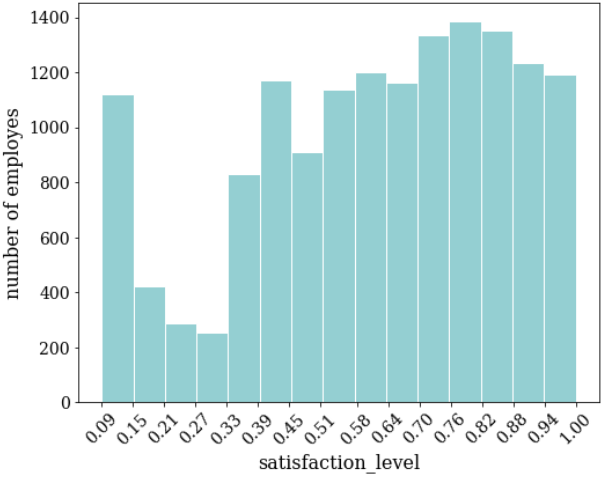
\includegraphics[height=4cm]{Images/Data_Understanding/Count/SL.png}
		\end{wrapfigure} 
		\paragraph{satisfaction\_level}$\newline$
		Type: Numerical Continuous $\newline$ Range: [0.09, 1] $\newline$
		Mean: 0.613 $\newline$
		Std: 0.249 $\newline$$\newline$
		La distribuzione è vicina ad una gaussiana sebbene sia leggermente sbilanciata per livelli di soddisfazione alti, come si nota anche dal valore della media, e abbia un picco iniziale. La variabile è stata discretizzata in 15 bins, calcolati tramite la regola di Sturges.
		
		\begin{wrapfigure}{l}{4.5cm}
			\vspace{-0.5cm}
			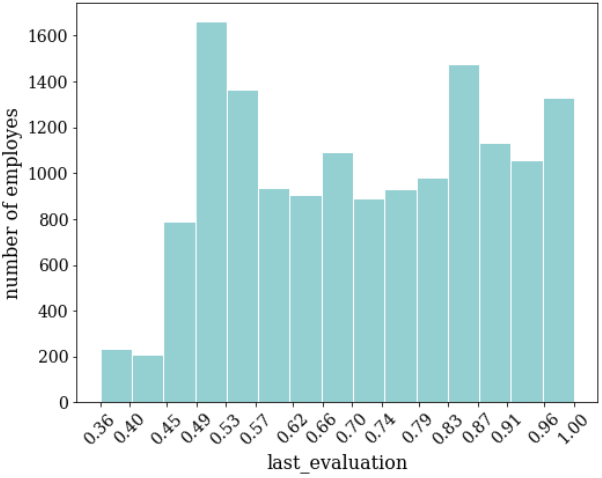
\includegraphics[height=4cm]{Images/Data_Understanding/Count/LE.png}
		\end{wrapfigure} 
		\paragraph{last\_evaluation}  $\newline$$\newline$
		Type: Numerical Continuous $\newline$ Range: [0.36, 1] $\newline$
		Mean: 0.716 $\newline$ Std: 0.171 $\newline$$\newline$
		Anche in questo caso possiamo assumere una distribuzione gaussiana ed utilizzare la regola di Sturges per suddividere la variabile in 15 bins. La distribuzione è piuttosto uniforme, sebbene vi siano un numero ristretto di impiegati che hanno ricevuto una valutazione molto bassa.
	\end{multicols}\vspace{0.2cm}
	\begin{multicols}{2}
		\begin{wrapfigure}{l}{4.5cm} 
			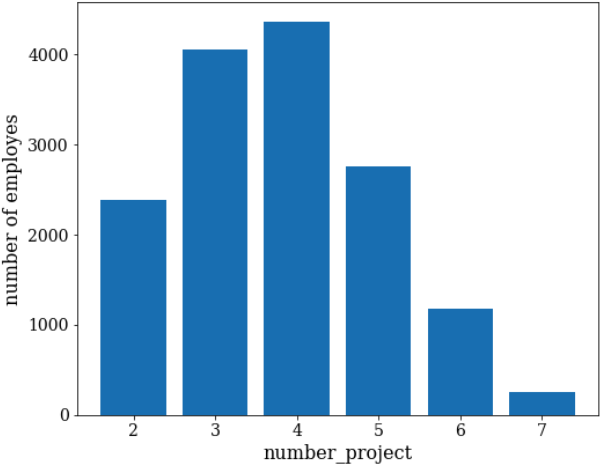
\includegraphics[height=3.9cm]{Images/Data_Understanding/Count/NP.png}
		\end{wrapfigure} 
		\paragraph{number\_project}$\newline$
		Type: Numerical Discrete$\newline$
		Range: [2, 7]$\newline$
		Mean: 3.803 $\newline$ Std: 1.233$\newline$$\newline$
		Il valore più frequente è 4, quello meno frequente è 7. Possiamo quindi notare che la maggior parte degli impiegati ha portato a termine dai 3 ai 5 progetti, mentre non vi sono impiegati che hanno svolti 0 o 1 progetto oppure più di 7.
	
		\begin{wrapfigure}{l}{4.5cm}
			\vspace{-0.5cm}
			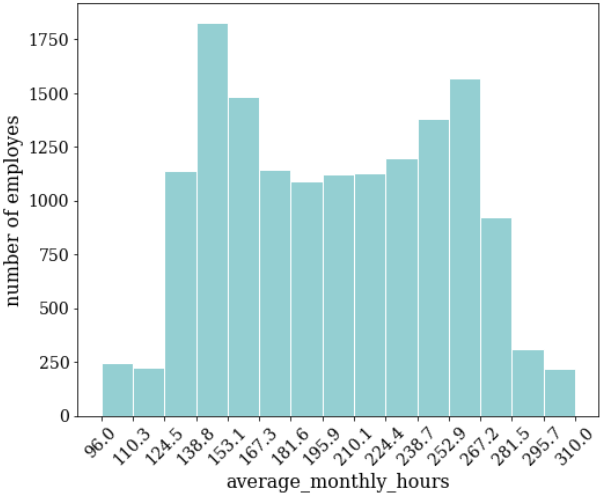
\includegraphics[height=4cm]{Images/Data_Understanding/Count/AMH.png}
		\end{wrapfigure} 
		\paragraph{average\_monthly\\ \_hours} $\newline$$\newline$
		Type: Numerical Discrete$\newline$ \hspace{1cm} Range: [96, 310]$\newline$
		Mean: 201.50 $\newline$ Std: 49.94$\newline$$\newline$
		La distribuzione di questa variabile è molto ben bilanciata in quanto è abbastanza simmetrica rispetto alla media. Poiché presentava troppi valori distinti si è deciso di discretezzare anche questa in 15 bins. 
		
	\end{multicols}\vspace{0.2cm}
	\begin{multicols}{2}
		
		\begin{wrapfigure}{l}{4.5cm} 
			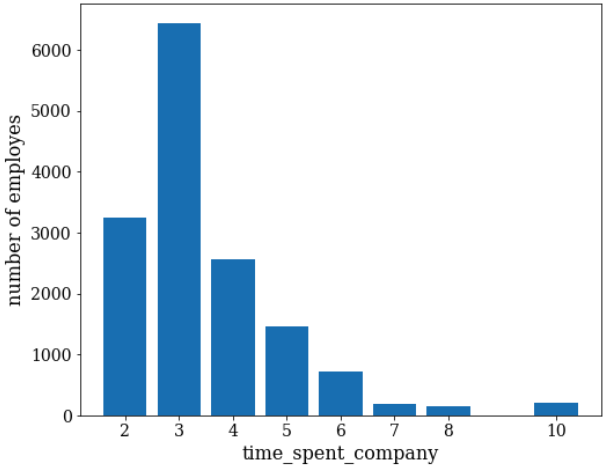
\includegraphics[height=3.9cm]{Images/Data_Understanding/Count/TSC.png}
		\end{wrapfigure} 
		\paragraph{time\_spent\\ \_company} $\newline$$\newline$
		Type: Numerical Discrete$\newline$
		Range: [2,10]$\newline$
		Mean: 3.498$\newline$ Std: 1.460$\newline$$\newline$
		\textit{time\_spent\_company} è una variabile fortemente sbilanciata che mostra la propensione dei dipendenti a rimanere nella compagnia per un periodo che va dai 2 ai 4 anni formando l’81.64\% del totale; coloro che invece rimangono dai 5 ai 7 anni sono il 15.86\%; il restante, che va da 8 a 10 anni è il 2,51\%.
		
		\begin{wrapfigure}{l}{4.5cm}
			\vspace{-0.5cm}
			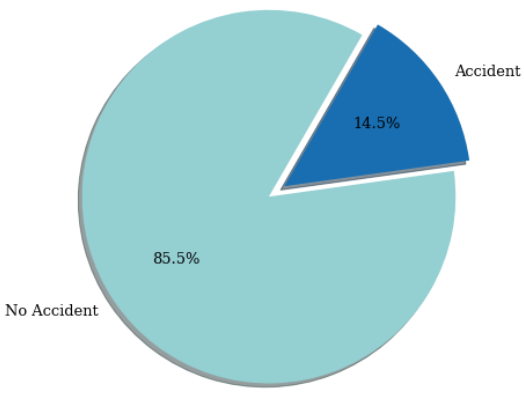
\includegraphics[height=3.9cm]{Images/Data_Understanding/Count/WA.png}
		\end{wrapfigure}
		\paragraph{work\_accident}$\newline$
		Type: Numerical Binary$\newline$
		Values: \{0,1\}$\newline$
		Mean: 0.145$\newline$ Std: 0.351$\newline$$\newline$
		La percentuale di incidenti sul lavoro è più alta di quanto si potrebbe pensare: il 14.5\% degli impiegati hanno avuto almeno un incidente. In ogni caso però l’attributo \textit{work\_accidents} risulta sbilanciato verso coloro che non hanno avuto incidenti  con l’87.5\% (12830 istanze) contro il 14.5\% del restante (2169 istanze) . 
	\end{multicols}\vspace{0.2cm}
	
	\begin{multicols}{2}
		
		\begin{wrapfigure}{l}{4.5cm} 
			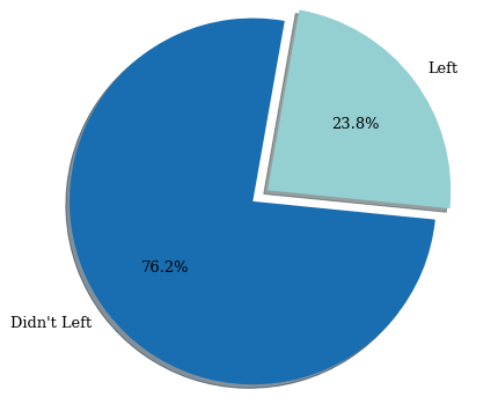
\includegraphics[height=4cm]{Images/Data_Understanding/Count/L.png}
		\end{wrapfigure} 
		\paragraph{left} $\newline$$\newline$
		Type: Numerical Binary$\newline$ Values: \{0, 1\}$\newline$
		Mean: 0.238 $\newline$ Std: 0.426$\newline$$\newline$
		\textit{left} sarà la nostra variabile di riferimento nel corso delle prossime analisi. La distribuzione non è equilibrata in quanto il 76.2\% (11428 istanze) delle persone ha deciso di restare nella compagnia a fronte del 23.8\% (3571 istanze) che ha invece deciso di lasciare.
		
		\begin{wrapfigure}{l}{4.5cm}
			\vspace{-0.5cm}
			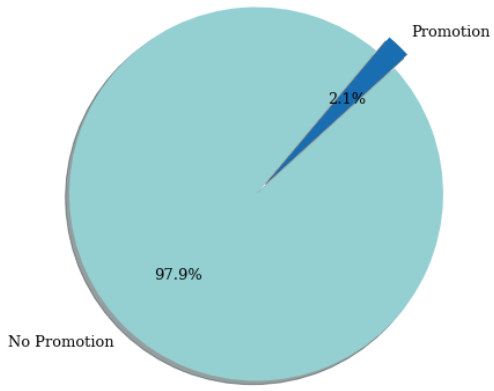
\includegraphics[height=4cm]{Images/Data_Understanding/Count/PL5Y.png}
		\end{wrapfigure} 
		\paragraph{promotion\_\\ last\_5years} $\newline$ $\newline$
		Type: Numerical Binary$\newline$
		Values: \{0, 1\}$\newline$
		Mean: 0.021 $\newline$ Std: 0.144	$\newline$$\newline$
		La variabile \textit{promotion\_last\_5years} è senza alcun dubbio la proprietà più sbilanciata con il 97.9\% (14680 istanze) di personale che non ha avuto una promozione negli ultimi 5 anni e con il restante 2.1\% (319 istanze) che è stato invece promosso.
		
	\end{multicols}
	$\newline$
	\begin{multicols}{2}
		
		\begin{wrapfigure}{l}{4.5cm} 
			\centering
			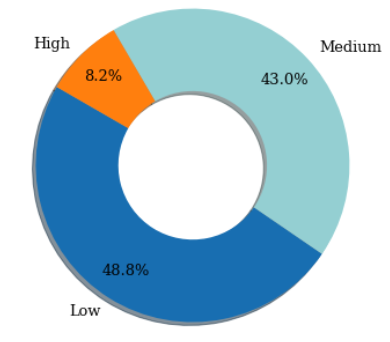
\includegraphics[height=3.7cm]{Images/Data_Understanding/Count/SY.png}
		\end{wrapfigure}
		\paragraph{salary}$\newline$$\newline$
		Type: Categorical$\newline$
		Values: \{Low, Medium, High\}$\newline$$\newline$
		La variabile \textit{salary} può assumere 3 valori che indicano la fascia di stipendio che gli impiegati percepiscono. La gran parte riceve uno stipendio medio-basso. In particolare il valore low racchiude il 48.8\% della popolazione, mentre medium il 43.0\%. Solo l'8.2\% degli impiegati ha uno stipendio che è considerato alto.
	
		\begin{wrapfigure}{l}{4.5cm}
			\vspace{-0.5cm}
			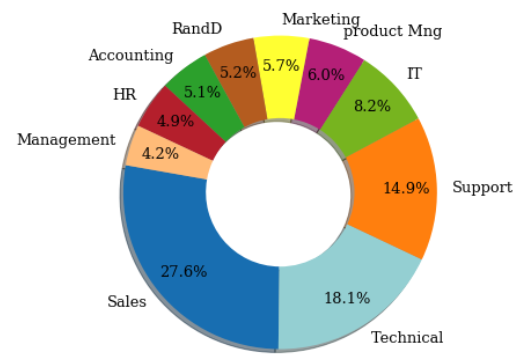
\includegraphics[height=3.5cm]{Images/Data_Understanding/Count/SS.png}
		\end{wrapfigure}
		\paragraph{departments}$\newline$$\newline$
		Type: Categorical$\newline$
		Values: \{sales, accounting, hr, technical, support, management, IT, product\_mng, marketing, RandD\}$\newline$$\newline$
		I dipartimenti con maggior numero di impiegati sono in ordine Sales, Technical, Support e IT. Gli altri sono approssimativamente distribuiti in modo uniforme. Il valore RandD indica il reparto di
		Research and Development.

	\end{multicols}
	
\subsection{Missing values e outliers}
	\begin{wrapfigure}{l}{10.5cm} 
		\vspace{-0.6cm}
		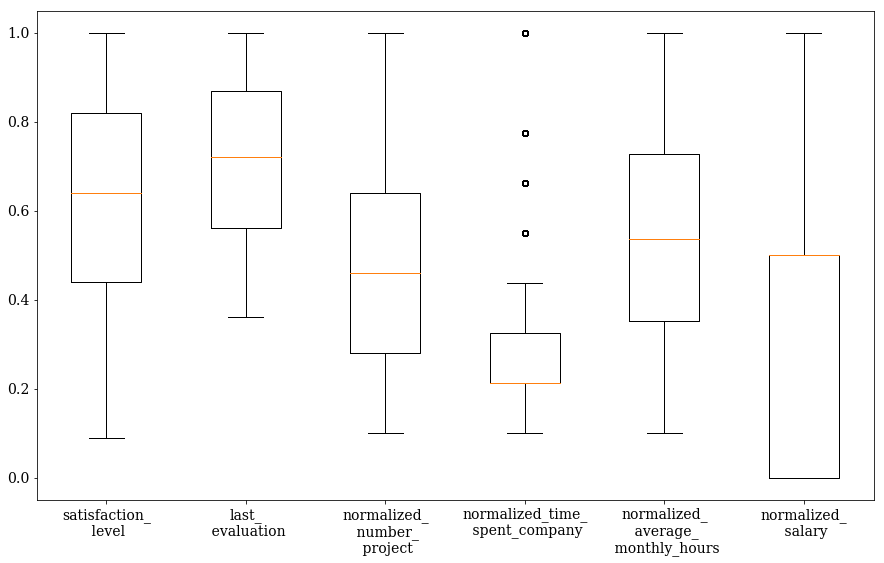
\includegraphics[height=7cm]{Images/Data_Understanding/BoxPlot.png}
		\vspace{-0.5cm}
		\caption{Box Plots.}
	\end{wrapfigure}
	Nel dataset non sono presenti missing values. Non è stata infatti rilevata la presenza esplicita di valori mancanti, né sono stati individuati valori di default che possano nascondere missing values.$\newline$
	Come mostrato dal grafico, è possibile individuare la presenza di alcuni outliers relativamente all’attributo \textit{time\_spent\_company}, che indica, in anni, da quanto tempo un impiegato lavora presso la compagnia. Gli outliers coincidono con i valori 6, 7, 8 e 10 che si allontanano significativamente dal resto dei valori.$\newline$
	Non è pensabile che tali valori costituiscano dati errati, ma si tratta semplicemente di dati che rispecchiano la situazione aziendale. Infatti è del tutto logico supporre che in un’azienda ci siano persone che lavorano da più tempo di altre, anche se in numero molto minore.$\newline$
	I record contenenti outliers sono in totale 1282. Si tratta circa dell’11,7\% dei record, che non sono pochi, ed inoltre, essi non incidono quasi per nulla sulla media e sulla standard deviation degli altri attributi. Per questi motivi, si è deciso di mantenerli all’interno del dataset.

\subsection{Discretizzazione e normalizzazione}
	Sono state applicate alle variabili del dataset alcune trasformazioni per poter processare e leggere più facilmente i dati.$\newline$
	Per poter applicare alcuni algoritmi che richiedono in input dati numerici, i valori degli attributi \textit{departments} e \textit{salary} sono stati trasformati da stringa a numero. 
	In particolare i dieci valori distinti di \textit{departments} (IT, RandD, accounting, hr, management, marketing, product\_mng, sales, support, technical) sono stati mappati rispettivamente con un valore numerico da 0 a 9, attraverso la creazione della nuova variabile \textit{departments\_val}.
	I tre valori di \textit{salary}, low, medium e high, sono stati mappati rispettivamente nei valori numerici 0, 1 e 2 all'interno della nuova variabile \textit{salary\_val}.$\newline$
	Per migliorare la leggibilità dei dati e ridurne la sparsità, è stata effettuata una discretizzazione delle variabili numeriche \textit{satisfaction\_level}, \textit{last\_evaluation} e \textit{average\_monthly\_hours}. Si è eseguito un natural binning per ottenere 15 bins con la stessa ampiezza. Il numero k di bins è stato scelto usando la formula di Sturges $k = \lceil 1+\frac{10}{3} log_{10} (N) \rceil$ in cui $ N $ è il numero totale dei valori dell'attributo (ovvero 14999).$\newline$
	In alcuni casi, per permettere un confronto più accurato tra variabili che hanno una scala diversa tra loro, sono stati normalizzati gli attributi \textit{number\_project}, \textit{time\_spent\_company} e \textit{average\_monthly\_hours} con una normalizzazione di tipo min-max in modo da trasformare i valori in una scala da 0 a 1, creando le nuove variabili \textit{normalized\_number\_project}, \textit{normalized\_time\_spent\_company}, \textit{normalized\_average\_monthly\_hours}.$\newline$
	Al fine di comprendere meglio il quantitativo medio di lavoro degli impiegati la variabile \textit{average\_monthly\_hours} è stata sostituita con \textit{average\_daily\_hours} , ottenuta dalla precedente tramite la seguente operazione:
	\begin{center}
		$\displaystyle \textit{average\_daily\_hours} = \frac{average\_monthly\_hours}{21.5}$
	\end{center}
	in cui possiamo assumere che in media vi siano 21.5 giorni lavorativi al mese. Tramite questa trasformazione otteniamo che gli impiegati lavorano in media $ 9.35 $ ore al giorno con una standard deviation di $ 2.32 $ ore. In questo modo quindi è stato più semplice comprendere che i turni di lavoro sono piuttosto lunghi.  Anche questa variabile, inoltre, è stata normalizzata con una normalizzazione di tipo min-max, ottenendo la nuova variabile \textit{normalized\_average\_daily\_hours}.
	

\subsection{Correlazioni tra le variabili}
	Nel database non sono presenti correlazioni sufficientemente alte che potrebbero indicare la presenza di variabili ridondanti.
	\begin{wrapfigure}{r}{0cm}
		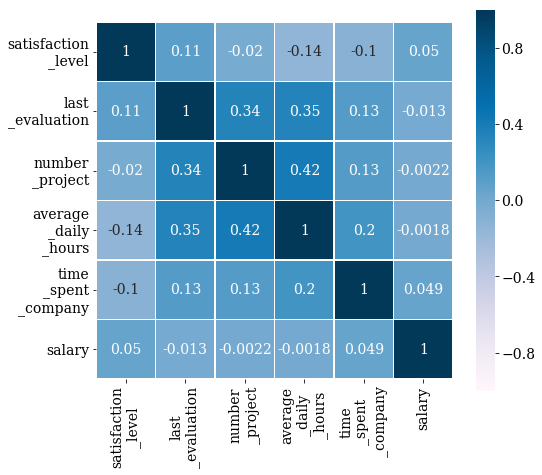
\includegraphics[height=8cm]{Images/Data_Understanding/Heatmap.png}
		\vspace{-0.5cm}
		\caption{Heatmap of correlation matrix.}
	\end{wrapfigure}	
	Utilizzando la formula di Pearson si può notare che c’è una leggera correlazione lineare positiva tra gli attributi \textit{last\_evaluation}, \textit{number\_project} e \textit{average\_daily\_hours}. Questo indica che al crescere di una anche le altre due tendono ad aumentare. \`{E} invece curioso notare che il livello di soddisfazione non è correlato a nessuno degli altri parametri. Oppure che il numero di progetti non aumenta in relazione al numero di anni passati nella compagnia, come ci si potrebbe aspettare.$\newline$
	Sono stati testati anche altri tipi di indici, tra cui Spearman, per valutare se la correlazione tra le variabili non fosse lineare ma non hanno portato a risultati significativamente diversi.$\newline$
	Il discorso invece cambia se eseguiamo la stessa analisi separando gli impiegati che se ne sono andati da quelli che sono rimasti (vedi figura 3) . Infatti, mentre nel primo gruppo le correlazioni diventano più evidenti e ne appaiono anche di nuove, nel secondo si annullano completamente.$\newline$
	Studiando il database così suddiviso si comprende che la leggera correlazione tra  \textit{last\_evaluation}, \textit{number\_project} e \textit{average\_monthly\_hours} che si era notata in precedenza è in realtà formata da una forte correlazione in quelli che hanno lasciato e una nulla negli altri. Inoltre, tra i lavoratori che hanno lasciato, è presente anche una correlazione positiva tra \textit{time\_spent\_company} e tutti gli altri attributi tranne salary. Questi schemi che si creano ci potrebbero aiutare anche in seguito per identificare quali impiegati se ne andranno. Infatti, se troviamo un record che presenta la stessa relazione tra le variabili che abbiamo appena descritto, potrebbe essere una prima indicazione che quella persona se ne potrebbe andare.$\newline$
	La popolazione di dipendenti ancora in azienda invece è più eterogenea, le variabili sono tutte indipendenti tra loro.
	\begin{center}
		\begin{tabular}{cc}
			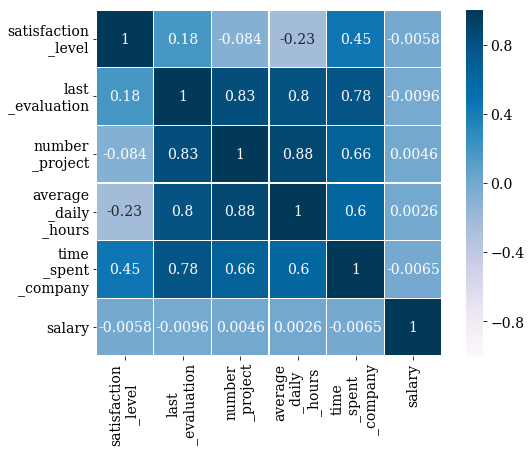
\includegraphics[width=0.4\linewidth]{Images/Data_Understanding/Heatmap_left.png} &
			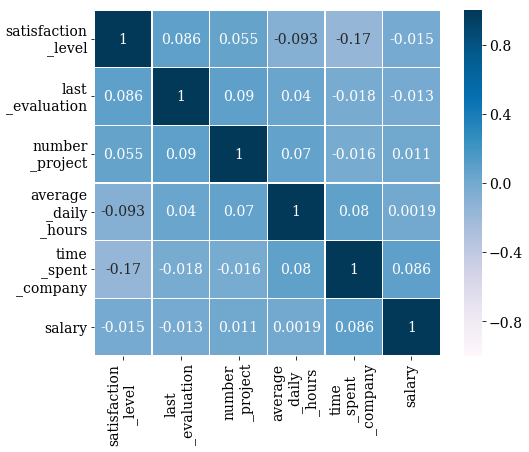
\includegraphics[width=0.4\linewidth]{Images/Data_Understanding/Heatmap_didnt_left.png} \\
			a) & b)\\
		\end{tabular}
		\vspace{-0.2cm}
		\captionof{figure}{Heatmap di chi ha lasciato (a) e di chi è rimasto (b).}
	\end{center}
